\documentclass[spec, och, otchet, hidelinks]{SCWorks}
% параметр - тип обучения - одно из значений:
%    spec     - специальность
%    bachelor - бакалавриат (по умолчанию)
%    master   - магистратура
% параметр - форма обучения - одно из значений:
%    och   - очное (по умолчанию)
%    zaoch - заочное
% параметр - тип работы - одно из значений:
%    otchet
%    referat    - реферат
%    coursework - курсовая работа (по умолчанию)
%    diploma    - дипломная работа
%    pract      - отчет по практике
%    pract      - отчет о научно-исследовательской работе
%    autoref    - автореферат выпускной работы
%    assignment - задание на выпускную квалификационную работу
%    review     - отзыв руководителя
%    critique   - рецензия на выпускную работу
% параметр - включение шрифта
%    times    - включение шрифта Times New Roman (если установлен)
%               по умолчанию выключен
\usepackage[T2A]{fontenc}
\usepackage[utf8]{inputenc}
\usepackage{graphicx}

\usepackage[sort,compress]{cite}
\usepackage{amsmath}
\usepackage{amssymb}
\usepackage{amsthm}
\usepackage{fancyvrb}
\usepackage{longtable}
\usepackage{array}
\usepackage[english,russian]{babel}
\usepackage{minted}
% Используется автором репозитория
%\usemintedstyle{xcode}
% Этот пакет включает в себя аналогичный Times New Roman шрифт.
% Необходим для успешной компиляции для UNIX-систем ввиду отсутствия TNR в нем.
% Можно использовать и для Windows.
\usepackage{tempora}


\usepackage[colorlinks=false]{hyperref}

\graphicspath{{figures/}}

\newcommand{\eqdef}{\stackrel {\rm def}{=}}

\newtheorem{lem}{Лемма}

% % При использовании biblatex вместо bibtex
%\usepackage[style=gost-numeric]{biblatex}
%\addbibresource{thesis.bib}

\begin{document}

% Кафедра (в родительном падеже)
\chair{математической кибернетики и компьютерных наук}

% Тема работы
\title{Логические элементы и схемы}

% Курс
\course{3}

% Группа
\group{331}

% Факультет (в родительном падеже) (по умолчанию "факультета КНиИТ")
%\department{факультета КНиИТ}

% Специальность/направление код - наименование
%\napravlenie{02.03.02 "--- Фундаментальная информатика и информационные технологии}
%\napravlenie{02.03.01 "--- Математическое обеспечение и администрирование информационных систем}
%\napravlenie{09.03.01 "--- Информатика и вычислительная техника}
%\napravlenie{09.03.04 "--- Программная инженерия}
\napravlenie{10.05.01 "--- Компьютерная безопасность}

% Для студентки. Для работы студента следующая команда не нужна.
%\studenttitle{Студентки}

% Фамилия, имя, отчество в родительном падеже
\author{Бородина Артёма Горовича}

% Заведующий кафедрой
\chtitle{доцент, к.\,ф.-м.\,н.} % степень, звание
\chname{С.\,В.\,Миронов}

%Научный руководитель (для реферата преподаватель проверяющий работу)
\satitle{аспирант}%, к.\,ф.-м.\,н.} %должность, степень, звание
\saname{А.\,А.\,Мартышкин}

% Руководитель практики от организации (только для практики,
% для остальных типов работ не используется)
\patitle{к.\,ф.-м.\,н., доцент}
\paname{Д.\,Ю.\,Петров}

% Семестр (только для практики, для остальных
% типов работ не используется)
\term{2}

% Наименование практики (только для практики, для остальных
% типов работ не используется)
\practtype{учебная}

% Продолжительность практики (количество недель) (только для практики,
% для остальных типов работ не используется)
\duration{2}

% Даты начала и окончания практики (только для практики, для остальных
% типов работ не используется)
\practStart{01.07.2016}
\practFinish{14.07.2016}

% Год выполнения отчета
\date{2022}

\maketitle

% Включение нумерации рисунков, формул и таблиц по разделам
% (по умолчанию - нумерация сквозная)
% (допускается оба вида нумерации)
%\secNumbering


\tableofcontents

% Раздел "Обозначения и сокращения". Может отсутствовать в работе
% \abbreviations
% \begin{description}
%     \item ... "--- ...
%     \item ... "--- ...
% \end{description}

% Раздел "Определения". Может отсутствовать в работе
%\definitions

% Раздел "Определения, обозначения и сокращения". Может отсутствовать в работе.
% Если присутствует, то заменяет собой разделы "Обозначения и сокращения" и "Определения"
%\defabbr


% Раздел "Введение"

\intro

\par Целью данной лабораторной работы служит ознакомление с основными характеристиками логических 
элементов и основами синтеза логических схем, изучение простейших комбинационных логических
устройств, реализующих логические функции сложения, умножения и отрицания.

\newpage

\section*{Задание 1.}
\addcontentsline{toc}{section}{Задание 1}

\par Запустить лабораторный комплекс Labworks и среду МS10 . Открыть файл \textbf{29.2.ms10}, 
размещенный в папке \textbf{Circuit Design Suitе 10.0} среды МS10, или собрать на рабочем поле 
среды MS10 схему для испытания \textit{основных и базовых логических элементов} и установить в 
диалоговых окнах компонентов их параметры или режимы работы. Скопировать схему в отчет.

\begin{figure}[h]
	\center{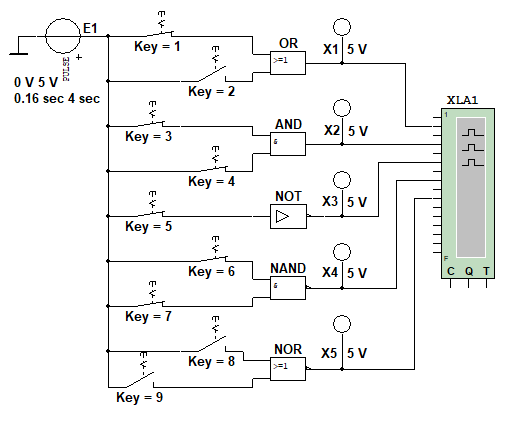
\includegraphics{circuit.png}}
	\caption{Схема с основными и базовыми логическими элементами.}
\end{figure}

\newpage

\par Оперируя ключами $ 1, 2, \dots, 9, $ сформировать все возможные комбинации аргументов $ x_1 $ 
и  $ x_2 $  (00, 10, 01 и 11) на входе дизъюнктора (\textbf{OR}), конъюнктора (\textbf{AND}), 
штриха Шеффера (\textbf{NAND}) и стрелки Пирса (\textbf{NOR}) и записать значения выходных 
логических функций $ y_k $ (0 или 1) в таблицу.

\begin{table}[h]
	\captionsetup{justification=centering}
	\begin{tabular}{|c|c|c|c|c|c|c|c|c|c|c|c|c|c|}	
		\hline	
		\multicolumn{3}{|c|}{[\textbf{OR}]} & \multicolumn{3}{|c|}{[\textbf{AND}]} & 
		\multicolumn{2}{|c|}{[\textbf{NOT}]} & \multicolumn{3}{|c|}{[\textbf{NAND}]} &
		\multicolumn{3}{|c|}{[\textbf{NOR}]} \\
		\hline
		$ \; x_1 \; $ & $ \; x_2 \; $ & $ \; y \; $ & $ \; x_1 \; $ & $ \; x_2 \; $ & $ \; y \; $ 
		& $ \; x \; $ & $ \; y \; $ & $ \; x_1 \; $ & $ \; x_2 \; $ & $ \; y \; $ & $ \; x_1 \; $ 
		& $ \; x_2 \; $ & $ \; y \; $ \\
		\hline
		0 & 0 & 0 & 0 & 0 & 0 & 0 & 1 & 0 & 0 & 1 & 0 & 0 & 1 \\
		\hline
		0 & 1 & 1 & 0 & 1 & 0 & 0 & 1 & 0 & 1 & 1 & 0 & 1 & 0 \\
		\hline
		1 & 0 & 1 & 1 & 0 & 0 & 1 & 0 & 1 & 0 & 1 & 1 & 0 & 0 \\
		\hline
		1 & 1 & 1 & 1 & 1 & 1 & 1 & 0 & 1 & 1 & 0 & 1 & 1 & 0 \\
		\hline	
	\end{tabular}
	\caption{Таблица истинности основных и базовых логических операций.}
\end{table}

\newpage

\section*{Задание 2.}
\addcontentsline{toc}{section}{Задание 2}

\par Собрать схему для реализации логической функции $ y $ с тремя аргументами $ a, b $ и $ c. $
Скопировать собранную логическую схему в отчет. Функция $ y $ имеет вид: $ y = (a + b + \neg c)
(\neg a + \neg b c)(a + \neg b + \neg c) $ (вариант \textnumero 2).

\begin{figure}[h]
	\center{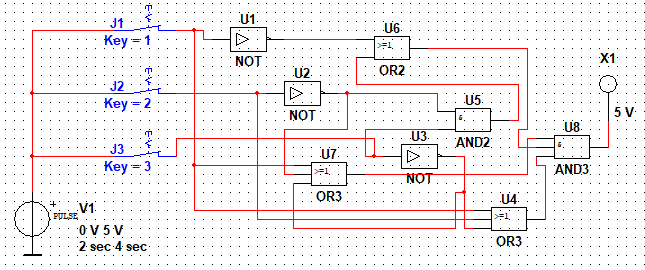
\includegraphics{my_circuit.png}}
	\caption{Схема заданной логической функции.}
\end{figure}

\begin{table}[h]
	\captionsetup{justification=centering}
	\begin{tabular}{|c|c|c|c|c|c|c|c|c|c|c|c|c|}
		\hline
		\multicolumn{4}{|c|}{$ y_1 = a + b + \neg c $} & \multicolumn{4}{|c|}{$ y_2 = \neg a + \neg b c $} & 
		\multicolumn{4}{|c|}{$ y_3 = a + \neg b + \neg c $} & $ y = y_1 \wedge y_2 \wedge y_3 $ \\
		\hline
		$ \; a \; $ & $ \; b \; $ & $ \; c \; $ & $ \; y_1 \; $ & 
		$ \; a \; $ & $ \; b \; $ & $ \; c \; $ & $ \; y_2 \; $ &
		$ \; a \; $ & $ \; b \; $ & $ \; c \; $ & $ \; y_3 \; $ &
		$ y $ \\
		\hline
		0 & 0 & 0 & 1 & 0 & 0 & 0 & 1 & 0 & 0 & 0 & 1 & 1 \\
		\hline
		0 & 0 & 1 & 0 & 0 & 0 & 1 & 1 & 0 & 0 & 1 & 1 & 0 \\
		\hline
		0 & 1 & 0 & 1 & 0 & 1 & 0 & 1 & 0 & 1 & 0 & 1 & 1 \\
		\hline
		0 & 1 & 1 & 1 & 0 & 1 & 1 & 1 & 0 & 1 & 1 & 0 & 0 \\
		\hline
		1 & 0 & 0 & 1 & 1 & 0 & 0 & 0 & 1 & 0 & 0 & 1 & 0 \\
		\hline
		1 & 0 & 1 & 1 & 1 & 0 & 1 & 1 & 1 & 0 & 1 & 1 & 1 \\
		\hline
		1 & 1 & 0 & 1 & 1 & 1 & 0 & 0 & 1 & 1 & 0 & 1 & 0 \\
		\hline
		1 & 1 & 1 & 1 & 1 & 1 & 1 & 0 & 1 & 1 & 1 & 1 & 0 \\
		\hline
	\end{tabular}
	\caption{Таблица истинности заданной логической функции.}
\end{table}

\newpage

% функция Пирса = 1 ттт x1 = x2 = 0 nor \\
% функция шеффера = 0 ттт x1 = x2 = 1 nand

%\section*{Перечень приборов, использованных в экспериментах.}
%\addcontentsline{toc}{section}{Перечень приборов, использованных в экспериментах}

%\par В ходе лабораторной работы использовались следующие приборы: 
%\par \textbf{Генератор прямоугольных сигналов} $ V_1 $ с амплитудой $ E $ = 5 B, длительностью импульса
%$ t_u $ = 2 с и периодом $ T $ = 4 с.
%\par \textbf{Три ключа}: $ J_1, J_2, J_3 $.
%\par \textbf{Три инвертора} NOT ($ U_1, U_2, U_3 $) для получения инверсий $ \neg a, \neg b, \neg c $.
%\par \textbf{Три дизъюнктора}: OR2 для реализации функции $ y_2 = \neg a + \neg bc $ и два OR3 для реализации
%функций $ y_1 = a + b + \neg c $ и $ y_3 = a + \neg b + \neg c $.
%\par \textbf{Два конъюнктора}: AND2 для реализации функции $ \neg b c $ и AND3 для реализации функции 
%$ y = y_1 \wedge y_2 \wedge y_3 $.
%\par \textbf{Пробник} X1 с пороговым напряжением 5 В. 

\newpage

\section*{Тестовые задания.}
\addcontentsline{toc}{section}{Тестовые задания}

1. Укажите \textbf{признаки}, характеризующие основные логические элементы:
\par $ \square \; $ на входах логических элементов аналоговые сигналы, а на выходах – цифровые: 
\textbf{неверно.} Как на входах, так и на выходах логических элементов сигналы цифровые, а именно
\textbf{бинарные.}

\par $ \square \; $ операции логического сложения, логического умножения и инверсия не составляют 
функционально полный набор: \textbf{неверно.} Операции $ y = x_1 + x_2, \; y = x_1 x_2, \; y = \bar x $
обладают функциональной полнотой и составляют функционально полный набор.

\par $ \square \; $ используя основные логические операции И, ИЛИ и НЕ, можно аналитически
выразить любую сложную логическую функцию: \textbf{верно.} Основные логические операции ИЛИ, И и НЕ 
позволяют аналитически описать, а логические элементы ИЛИ (дизъюнктор), И (конъюнктор) и НЕ (инверсор) - 
реализовать комбинационное устройство любой степени сложности.

\par $ \square \; $ минимальный логический базис составляют операции ИЛИ и НЕ или И и НЕ: \textbf{верно.}
Используя законы де Моргана, можно выразить конъюнкцию через дизъюнкцию и три отрицания. 
Аналогично можно выразить дизъюнкцию: $$ a \wedge b = \neg(\neg a \vee \neg b), \quad 
a \vee b = \neg(\neg a \wedge \neg b) $$

\par $ \square \; $ входные и выходные сигналы логических элементов могут принимать только
два значения: логическую 1 и логический 0: \textbf{верно.}
\par $ \square \; $ операция логического сложения совпадает с операцией обычного сложения. \textbf{неверно.}
Равенство выполняется только в том случае, когда либо оба операнда равны нулю, либо один равен нулю, 
а второй единице.

2. Укажите \textbf{выражение} логической функции двух переменных $ x_1 $ и $ x_2 $, реализуемой элементом
<<стрелка Пирса>>: $ y = \overline{x_1 + x_2} $

3. Укажите \textbf{выражение} логической функции двух переменных $ x_1 $ и $ x_2 $, реализуемой элементом
<<штрих Шеффера>>: $ y = \overline{x_1 x_2} $

4. Укажите \textbf{выражение} логической функции трех переменных $ a, b $ и $ c $, записанной в совершенной
дизъюнктивной нормальной форме (СДНФ): $ y(a, b, c) = \bar a bc + a \bar b c + ab \bar c + abc $.

5. Укажите \textbf{элемент} ИЛИ-НЕ:

\begin{figure}[h]
	\center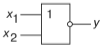
\includegraphics{nor.png}
	\caption{Элемент ИЛИ-НЕ.}
\end{figure}

6. Укажите \textbf{элемент} И:

\begin{figure}[h]
	\center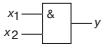
\includegraphics{and.png}
	\caption{Элемент ИЛИ-НЕ.}
\end{figure}

7. Укажите значение \textbf{функции} $ y = (ab + \bar c)(\bar a + \bar b) $, если $ a = b = c = 1 $: \textbf{0}.

\newpage

\conclusion

\par В ходе лабораторной работы мы ознакомились с основными характеристиками логических элементов и 
основами синтеза логических схем на примере построения простейшей электросхемы и составления для неё 
таблицы истинности. Также нами были рассмотрены и изучены простейшие комбинационные логические устройства,
реализующие логические функции сложения, умножения и отрицания.

\newpage

\end{document}

% После введения — серии \section, \subsection и т.д.


% Раздел "Заключение"
\conclusion

%Библиографический список, составленный вручную, без использования BibTeX
%
%\begin{thebibliography}{99}
%  \bibitem{Ione} Источник 1.
%  \bibitem{Itwo} Источник 2
%\end{thebibliography}

%Библиографический список, составленный с помощью BibTeX
%
\bibliographystyle{gost780uv}
\bibliography{thesis}

% % При использовании biblatex вместо bibtex
%\printbibliography

% Окончание основного документа и начало приложений
% Каждая последующая секция документа будет являться приложением
\appendix

\end{document}